
\chapter{Application: Jakobshavn} \label{ssn_application_jakobshavn}

\begin{figure}
  \centering
    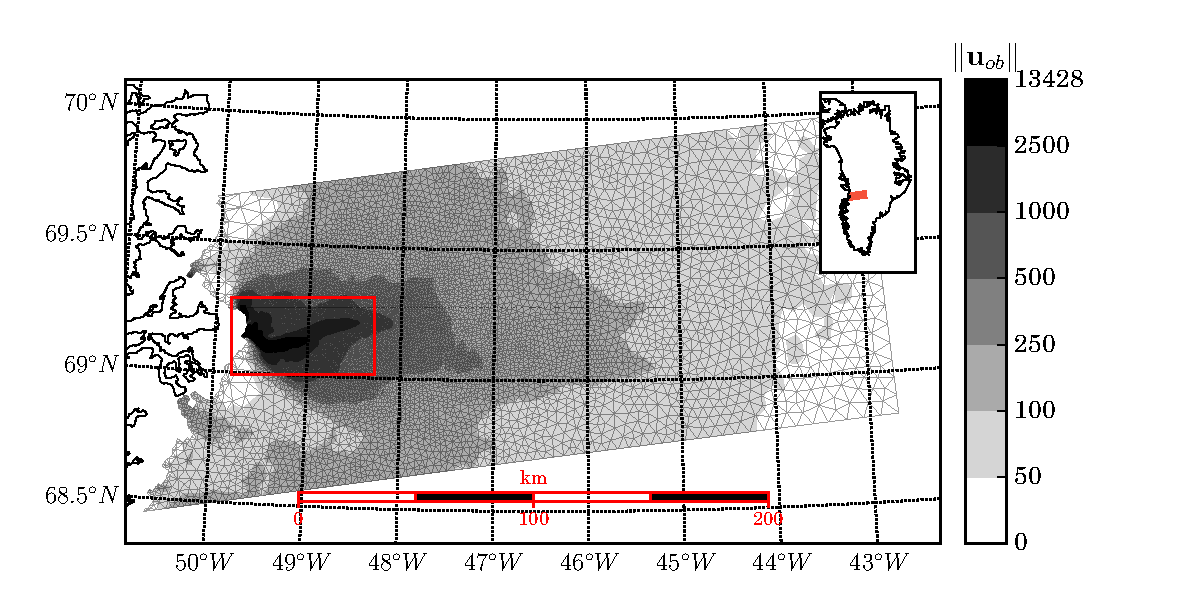
\includegraphics[width=\linewidth]{images/internal_energy/jakob_results/inversion_Wc_0.01/region.pdf}
  \caption[Jakobshavn Glacier mesh]{Surface velocity magnitude observations in m a\sups{-1} from \citet{rignot_2012} over the Jakobshavn region highlighted in {\color[RGB]{245, 81, 58}orange} in the inlaid map.}
  \label{jakobshavn_region}
\end{figure}

\begin{figure*}
  \centering
    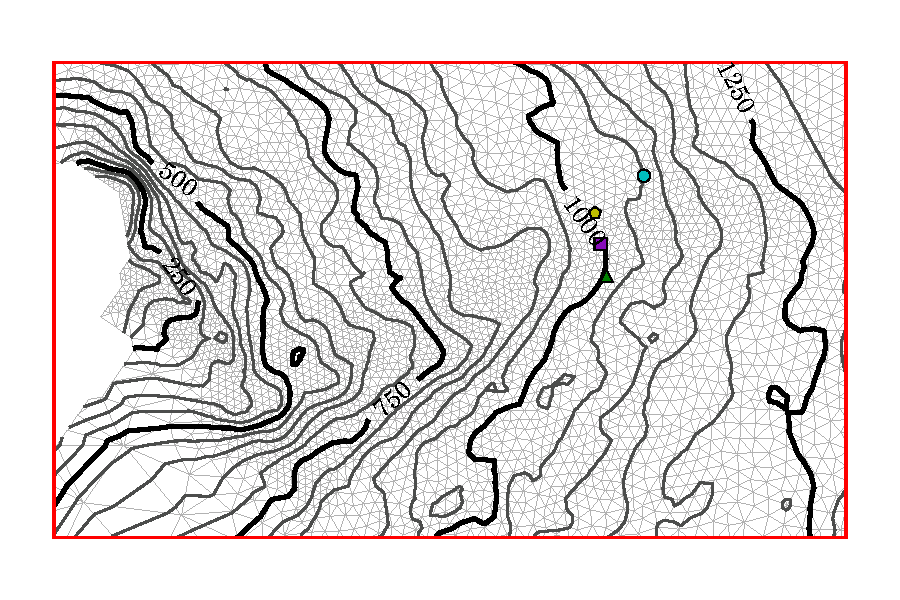
\includegraphics[width=0.8\linewidth]{images/internal_energy/jakob_results/inversion_Wc_0.01/S.pdf}
    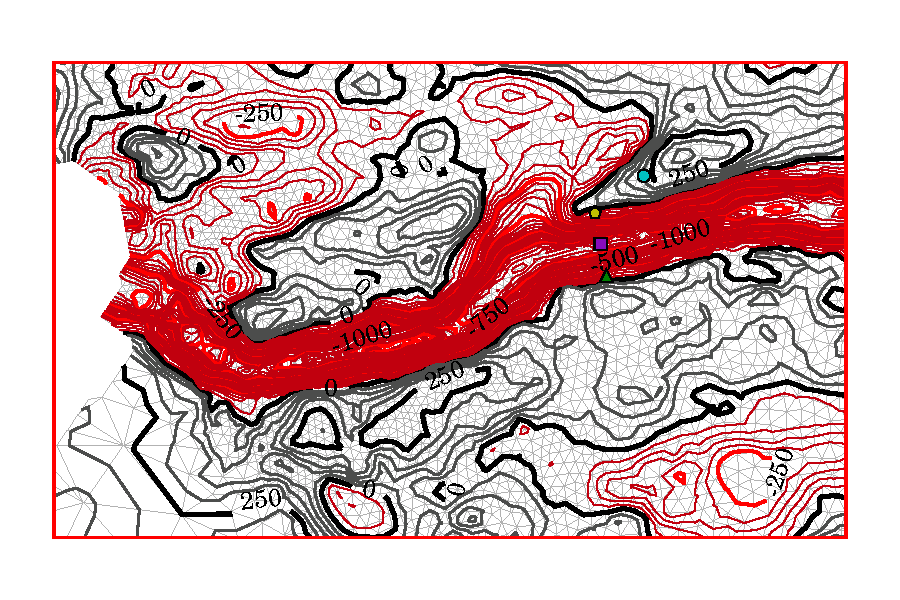
\includegraphics[width=0.8\linewidth]{images/internal_energy/jakob_results/inversion_Wc_0.01/B.pdf}
  \caption[Jakobshavn Glacier topography]{Topography of surface $S$ in m (top) and basal topography in m (bottom) provided by \citet{bamber_2013} for the rectangular region outlined in {\color{red}red} in Figure \ref{jakobshavn_region}.  Topography contours are spaced 50 m, with negative heights colored {\color{red}red}.  The colored points roughly correspond to the locations examined by \citet{luethi_2002}.}
  \label{jakobshavn_topography}
\end{figure*}

\index{Non-linear differential equations!3D}

The region surrounding Jakobshavn Glacier was chosen to test the applicability of the methods of Chapters \ref{ssn_momentum_and_mass_balance}, \ref{ssn_internal_energy_balance}, and \ref{ssn_inclusion_of_velocity_data} to real-world data.  To simplify computations while simultaneously producing high-resolution results, the domain was restricted to a rectangular region with Eastern-most boundary located close to the divide, with an along-flow width of approximately 120 km.  A triangular mesh was first created with a minimum cell diameter of 500 m in the fastest-flowing regions and maximum cell diameter of 15 km in the slowest-flowing regions.  This mesh was then extruded vertically into ten layers of tetrahedra and deformed to match the geometry supplied by \citet{bamber_2013} (see Code Listing \ref{cslvr_jakobshavn_gen_mesh} and Figures \ref{jakobshavn_region} and \ref{jakobshavn_topography}).

In order to retain the well-posedness of thermo-mechanical system (\ref{energy_euler_lagrange}), (\ref{gamma_a_ebc} -- \ref{energy_flux}), (\ref{cons_momentum} - \ref{cons_mass}), and (\ref{surface_stress} -- \ref{impenetrability}), extra boundary conditions must be applied along the interior regions of ice having been cut by the specification of the mesh boundary, denoted $\Gamma_D$ (Figure \ref{ice_profile_domain}).  These extra conditions are
{\small
\begin{align}
  \label{gamma_d_stress}
  \sigma \cdot \normal &= - f_c \normal &&\text{ on } \Gamma_D &&\leftarrow \text{ full-Stokes cry'st'c str.} \\
  \label{gamma_d_bp_stress}
  \sigma_{\text{BP}} \cdot \normal &= \rankone{0} &&\text{ on } \Gamma_D &&\leftarrow \text{ first-order cry'st'c str.} \\
  \label{gamma_d_energy}
  \theta &= \theta_S &&\text{ on } \Gamma_D &&\leftarrow \text{ Dirichlet},
\end{align}}
with cryostatic stress $f_c$ defined by (\ref{exterior_pressure}).  As depicted by the $f_c \normal$ vectors in Figure \ref{ice_profile_domain}, full-Stokes stress condition (\ref{gamma_d_stress}) and first-order stress condition (\ref{gamma_d_bp_stress}) represent the contribution of stress presented to the ice column by the surrounding ice removed from the domain.

While it is unlikely that the energy is unchanging from the surface throughout the interior of the ice along the surface $\Gamma_D$ as stated by `Dirichlet' condition (\ref{gamma_d_energy}), the region of interest lies $\approx$ 75 km from this boundary, with very low velocity magnitude (Figure \ref{jakobshavn_region}).  Thus it is expected that the effect of this inconsistency is small.

To initialize the basal traction, we used the SIA approximate field $\beta_{\text{SIA}}$ described in \S \ref{ssn_dual_optimization}.  In order to initialize flow-rate factor (\ref{rate_factor}), the initial energy values $\theta^i$ throughout the interior $\Omega$ were initialized using quadratic energy (\ref{energy_quad}) with initial water content $W^i(z) = 0$ and surface temperatures $T^i(x,y,z) = T_S(x,y), \forall z$ provided by \citet{fausto_2009}.  Also, pressure melting temperature (\ref{temperature_melting}) requires that pressure $p$ be initialized; here we applied cryostatic pressure $f_c$ in (\ref{exterior_pressure}) such that $p^i(z) = f_c(z) = \rho g (S - z)$.  Finally, the basal-water discharge $F_b$ across the entire basal domain was initialized to zero.

The $L^2$ and logarithmic cost functional coefficients in (\ref{momentum_objective}), $\gamma_1$ and $\gamma_2$, respectively, were determined as described in \S \ref{ssn_ismip_hom_inverse_sims}; by completing Algorithm \ref{tmc_da} several times and adjusting their relative values such that at the end of the process their associated functionals were of approximately the same order (Figure \ref{convergence}).

An appropriate value for the regularization parameters $\gamma_3$ and $\gamma_4$ in momentum objective (\ref{momentum_objective}) was determined from an L-curve process (\S \ref{ssn_l_curve}).  First, it was noted that when performing this procedure for only one regularization term, \ie, setting one of either $\gamma_3$ or $\gamma_4$ to zero, this process resulted in choosing $\gamma_3 = \gamma_4 = 10$.  We then took $\gamma_4 = 10$ and increased $\gamma_3$ until the Tikhonov regularization functional began to affect the regularization of optimal traction $\beta^*$, resulting in choosing $\gamma_3 = 0.1$.

Finally, the geothermal heat flux was set to the average Greenland value of $\bar{q}_{geo} = 4.2 \times 10^{-2}$ W m\sups{-2} \citep{paterson_1994} so as to minimize its effect on basal melt rate (\ref{basal_melt_rate}) and hence also basal water discharge $F_b$ as expressed by basal energy flux (\ref{energy_flux}).  For a complete listing of initial variables and coefficients used, see Table \ref{initial_values}.  The \CSLVR scripts used to generate the mesh, data, and results are shown in Code Listings \ref{cslvr_jakobshavn_gen_mesh}, \ref{cslvr_jakobshavn_gen_data}, and \ref{cslvr_jakobshavn_da}, respectively.

\begin{table}
\centering
\caption[Jakobshavn simulation variables]{Initial values used for Jakobshavn sim's.}
\label{initial_values}
\begin{tabular}{llll}
\hline
\textbf{Variable} & \textbf{Value} & \textbf{Units}\footnote{All units including the dimension of time have been converted from per second to per annum in order to account for the very slow speed of ice.} & \textbf{Description} \\
\hline
$D$ & $0$ & m & ocean height \\
$q_{geo}$ & $4.2 \times 10\sups{-2}$ & W m\sups{-2} & geothermal heat flux \\
$\dot{\varepsilon}_0$ & $10\sups{-15}$ & a\sups{-1} & strain regularization \\
$\gamma_1$ & $5 \times 10^3$ & kg m\sups{-2}a\sups{-1} & $L^2$ cost coefficient \\
$\gamma_2$ & $10^{-2}$ & J a\sups{-1} & log. cost coefficient \\
$\gamma_3$ & $10^{-1}$ & m\sups{6}kg\sups{-1}a\sups{-1} & Tikhonov reg. coef. \\
$\gamma_4$ & $10$ & m\sups{6}kg\sups{-1}a\sups{-1} & TV reg. coeff. \\
$\theta^i$ & $\theta(T_S, 0)$ & J kg\sups{-1} & initial energy \\
$\beta^i$ & $\beta_{\text{SIA}}$ & kg m\sups{-2}a\sups{-1} & initial friction coef. \\
$F_b^i$ & $0$ & m a\sups{-1} & ini.~basal water flux \\
$p^i$   & $f_c$ & Pa & initial pressure \\
$k_0$   & $10^3$ & -- & energy flux coefficient \\
\end{tabular}
\end{table}

%===============================================================================
%===============================================================================

\section{Results}

The first set of results were generated using a maximum basal water content of $W_c = 0.01$, corresponding to the maximum observed in this area \citep{luethi_2002}.  To ensure convergence, Algorithm \ref{tmc_da} was run for 10 iterations using 1000 iterations of momentum barrier problem (\ref{momentum_barrier}) (Figure \ref{convergence}).

For each iteration of this simulation, the surface velocity mismatch between modeled results and observations supplied by \citet{rignot_2012} remained at least one order of magnitude lower than the surface speed, with greatest error near the terminus (Figure \ref{jakobshavn_results}).  As evident by Figure \ref{convergence}, both regularization functionals (\ref{tikhonov_regularization}, \ref{tv_regularization}) and the $L^2$ cost functional (\ref{l2_cost}) of momentum objective (\ref{momentum_objective}) reach approximately the same respective minimums at the end of each iteration, while the logarithmic cost functional (\ref{logarithmic_cost}) -- which is most affected by velocity mismatches in slower regions of flow distant from the terminus -- continues to decrease.  This may be due to the fact that for each iteration, both basal-melting rate $M_b$ and basal traction $\beta$ remain quite low near the region of fast flow nearest the terminus, and thus $L^2$ cost (\ref{l2_cost}) is little affected by changes in internal energy.

It was observed that for each iterative change in basal traction $\beta$ -- and thus also basal melt-rate (\ref{basal_melt_rate}) and internal friction (\ref{strain_heat}) -- the optimization procedure for basal-water discharge $F_b$ would reach a value required to flush out water generated by both of these sources.  As a result of this, at each iteration the basal water content remained close to $W_c$ and the vertically averaged water content $\bar{W}$ remained in all but a few areas below 5\% (Figure \ref{jakobshavn_results}).

The column percentage of temperate ice resulting from this simulation is on average about twice that reported by \citet{luethi_2002}, despite the imposition of an approximately 10$^{\circ}$ K lower surface temperature.  This is likely due to both the improper specification of the CTS constraints, as explained by \citet{blatter_2015}, and the low vertical resolution of the mesh (Figure \ref{jakobshavn_profile}).  The sharp decline in temperature near the surface, followed by the sharp increase at the next vertex of the mesh, suggests that the thermal gradient near the surface is creating numerical oscillations.  In such a case, increasing the vertical resolution of the mesh will reduce the instability and result in a higher-magnitude temperature gradient near the surface, hence reducing the temperature to a level closer to expectations.

Remarkably, nearly the entire column of ice is temperate along the shear margins nearest the terminus (Figure \ref{jakobshavn_results}).  As a result, basal traction $\beta$ must increase in order to compensate for the approximately three-fold enhancement of flow-rate factor (\ref{rate_factor}) and relatively low surface speed there.  Additionally, the basal water discharge optimization process does not appear to compensate for the relatively high basal water content of these regions; it may be necessary to append energy objective (\ref{energy_objective}) with an additional term favoring areas with largest misfit, similar to momentum objective (\ref{momentum_objective}).  Finally, we note that an entirely different ice-flow model applies to the shear margins due to the extreme levels of strain-heat and damaged ice in this region.

For an additional test, the data-assimilation process described by Algorithm \ref{tmc_da} was performed once more for ten iterations with two simulations; one using a maximum basal water content $W_c =0.03$ and one using $W_c = 0.01$, in the hope of comparison.  The ratio of basal traction fields derived using maximum water content $W_c = 0.01$ and $W_c = 0.03$ is shown in Figure \ref{deltas}.  While the traction appears to be up to six times greater along the main trench, it is important to note that the friction is quite small in this region (Figure \ref{jakobshavn_results}) and thus has little effect on the velocity field.  However, the traction along the flanks of the trench approximately 20 km inland are up to half has large when the maximum basal water content is reduced from 3\% to 1\%.  This may be explained by both the reduction in height of the CTS and the reduction in water content to a point below that required by the empirically-constrained water content relation $W_f$ in rate factor (\ref{rate_factor}).

\section{Conclusion}

The methods presented in \S \ref{ssn_water_content_optimization} and \S \ref{ssn_dual_optimization} offer a new approach to approximate the energy and momentum distributions of an ice-sheet or glacier.  This method, having been derived from established balance equations, provides the ability to match energy distributions to observations of internal-water content.  This method results in a consistent estimate of velocity, energy, basal-water discharge, and basal traction.  Applying this procedure over the region of Jakobshavn indicated that altering the maximum-allowed basal-water content has a significant effect on basal traction values derived by data-assimilation methods.

\pythonexternal[label=cslvr_jakobshavn_gen_mesh, caption={\CSLVR script used to generate the mesh for the Jakobshavn simulation.}]{scripts/jakobshavn/gen_jakobshavn_mesh_small_block.py}

\pythonexternal[label=cslvr_jakobshavn_gen_data, caption={\CSLVR script used to generate the data used by Code Listing \ref{cslvr_jakobshavn_da}.}]{scripts/jakobshavn/gen_jakobshavn_vars_small.py}

\pythonexternal[label=cslvr_jakobshavn_da, caption={\CSLVR script used to simultaneously assimilate data $\rankone{u}_{ob}$ and $W_c$.}]{scripts/jakobshavn/data_assimilation.py}

\pythonexternal[label=cslvr_jakobshavn_sb, caption={\CSLVR script used calculate the stress-balance for the Jakobshavn simulation results as depicted in Figures \ref{jakobshavn_membrane_stress} and \ref{jakobshavn_membrane_stress_balance}.}]{scripts/jakobshavn/stress_balance.py}

\pythonexternal[label=cslvr_jakobshavn_region, caption={\CSLVR script used generate Figures \ref{jakobshavn_region} and \ref{jakobshavn_topography}.}]{scripts/jakobshavn/plot_region.py}

\begin{figure*}
  \centering
    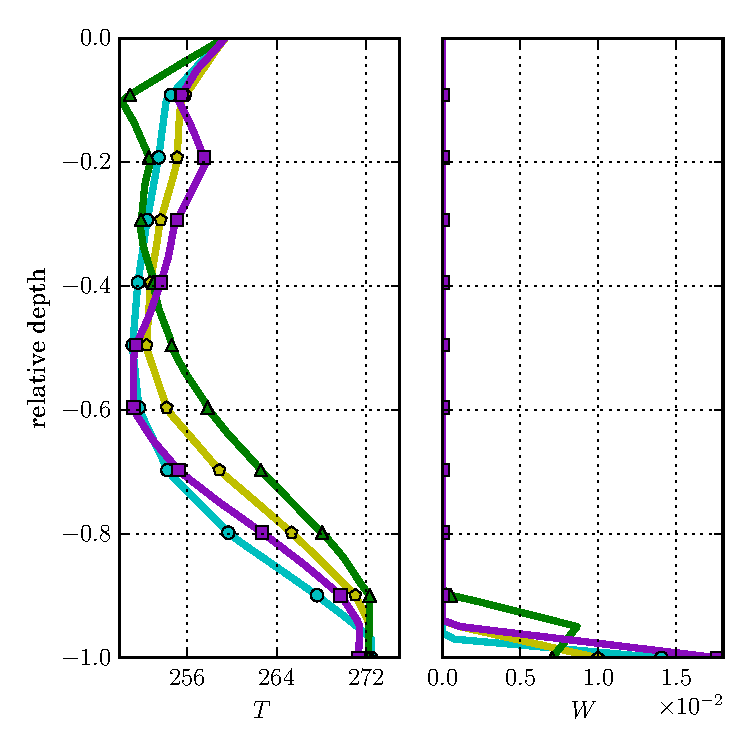
\includegraphics[width=0.48\linewidth]{images/internal_energy/jakob_results/inversion_Wc_0.01/profile_plot.pdf}
    \quad
    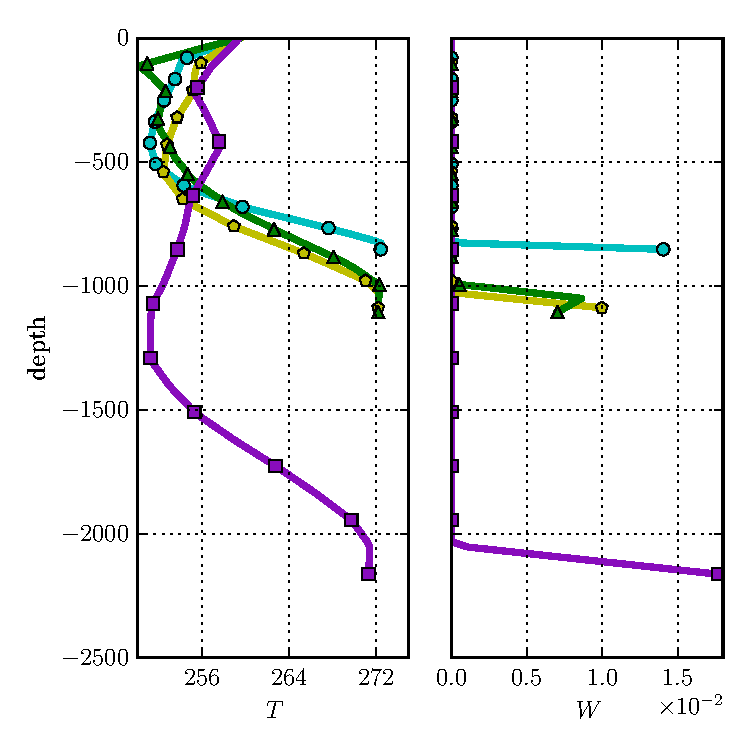
\includegraphics[width=0.48\linewidth]{images/internal_energy/jakob_results/inversion_Wc_0.01/profile_plot_depth.pdf}
  \caption[Jakobshavn energy profiles]{Temperature $T$ in degrees K and unit-less water content $W$ profiles with relative-depth-vertical coordinates (left) and actual depth coordinates (right).  The colored points correspond to the latitude/longitude coordinates in Figure \ref{jakobshavn_topography}, and the points indicate vertex locations of the mesh from which the data were interpolated.}
  \label{jakobshavn_profile}
\end{figure*}

\begin{figure*}
  \centering
    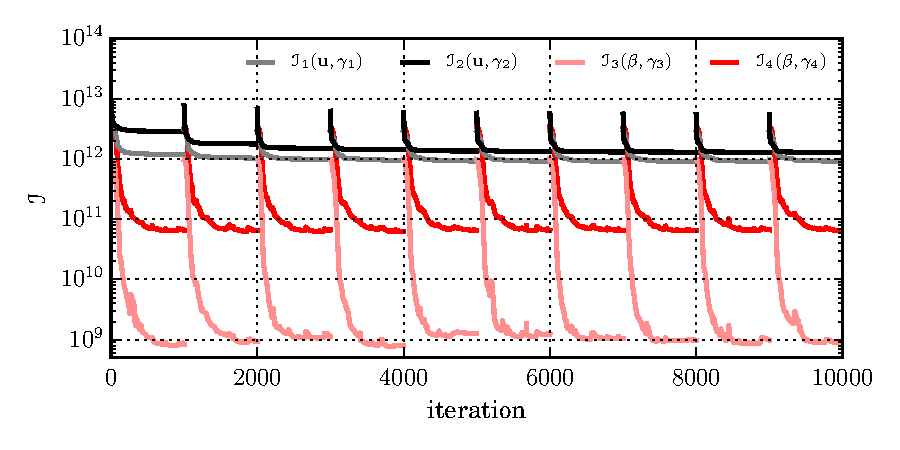
\includegraphics[width=\linewidth]{images/internal_energy/jakob_results/inversion_Wc_0.01/convergence_plot.pdf}
  \caption[Jakobshavn simulation convergence plot]{Convergence plots of momentum objective functional (\ref{momentum_objective}) for Algorithm \ref{tmc_da} using maximum basal water content $W_c = 0.01$.  The individual components include logarithmic cost functional (black), $L^2$ cost functional ({\color[RGB]{128,128,128}dark gray}), Tikhonov regularization functional ({\color[RGB]{255,142,142} light red}), and total variation regularization functional ({\color[RGB]{255,0,0}red}). The peaks located every 1000 iterations indicate iterations of Algorithm \ref{tmc_da}.}
  \label{convergence}
\end{figure*}

\begin{figure*}
  \centering
    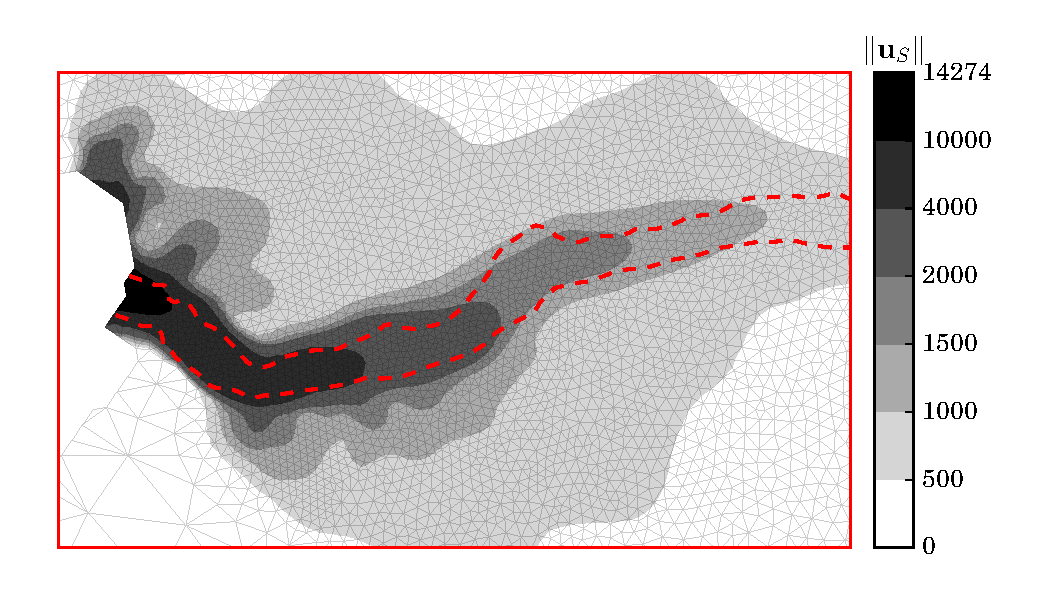
\includegraphics[width=0.48\linewidth]{images/internal_energy/jakob_results/inversion_Wc_0.01/U_mag.pdf}
    \quad
    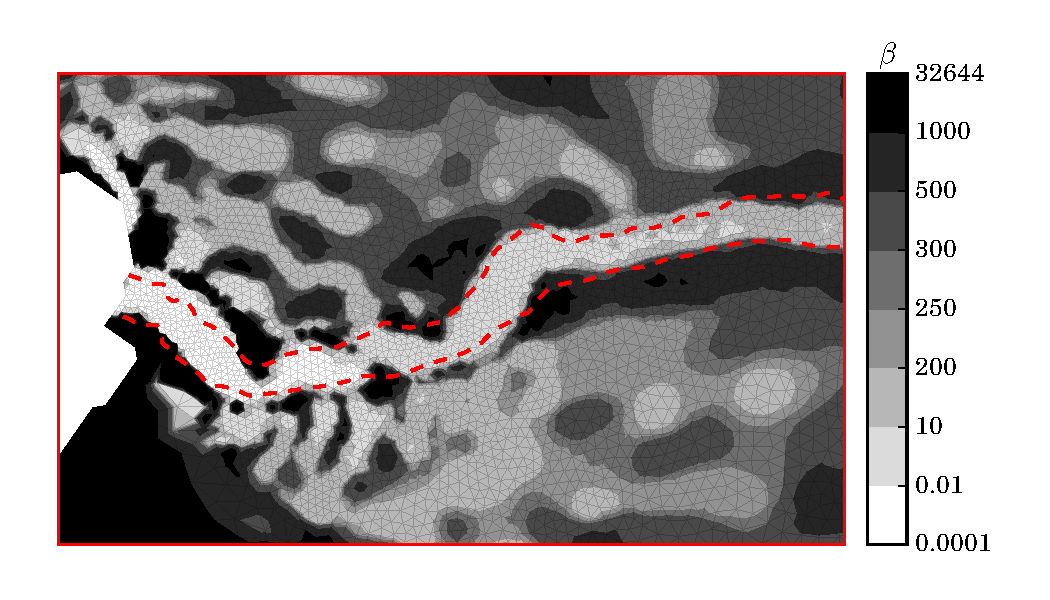
\includegraphics[width=0.48\linewidth]{images/internal_energy/jakob_results/inversion_Wc_0.01/beta.pdf}

    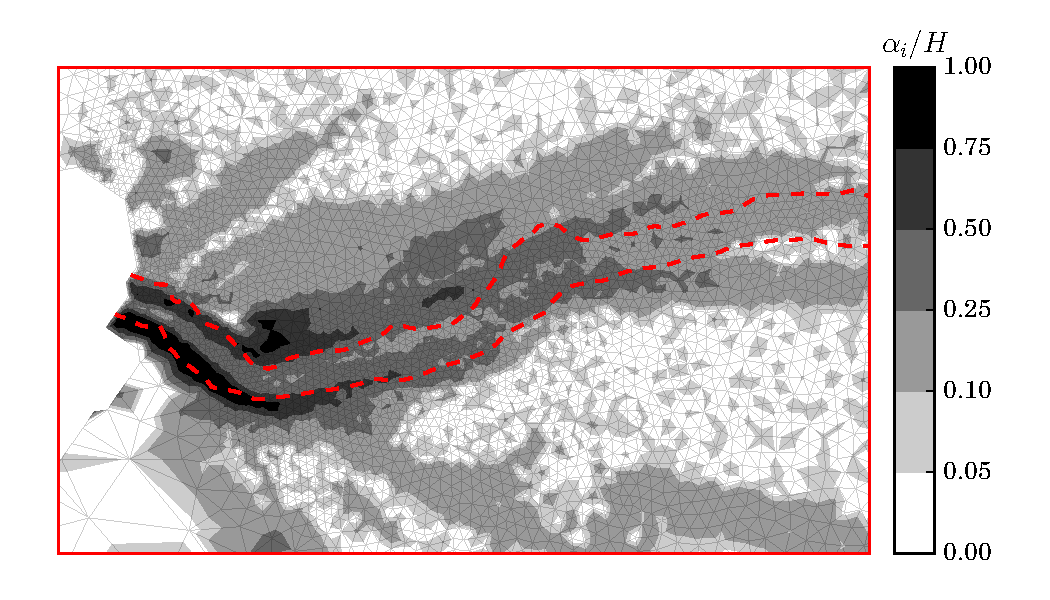
\includegraphics[width=0.48\linewidth]{images/internal_energy/jakob_results/inversion_Wc_0.01/temp_rat.pdf}
    \quad
    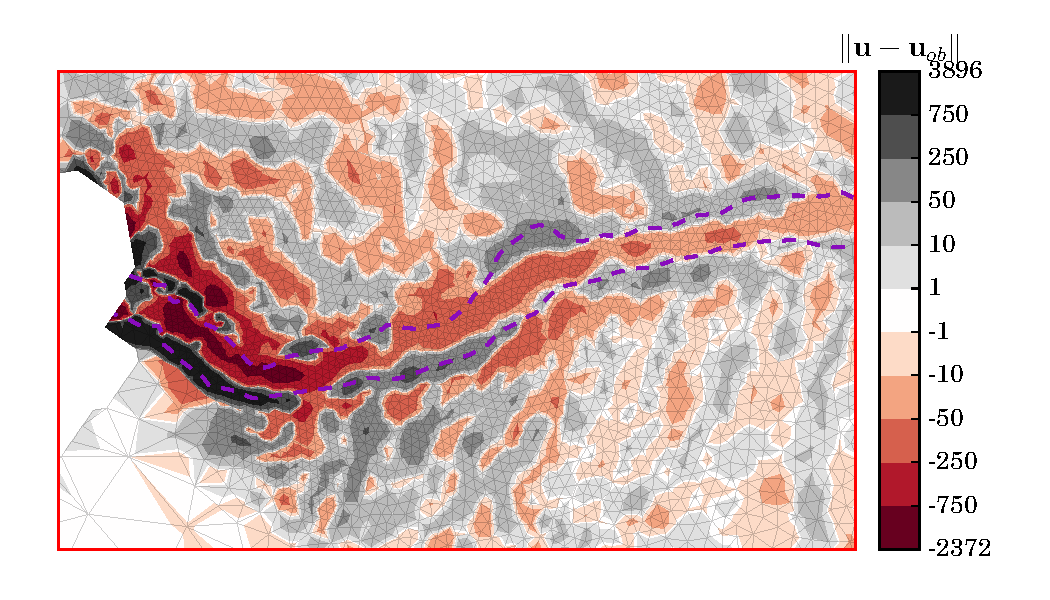
\includegraphics[width=0.48\linewidth]{images/internal_energy/jakob_results/inversion_Wc_0.01/misfit.pdf}

    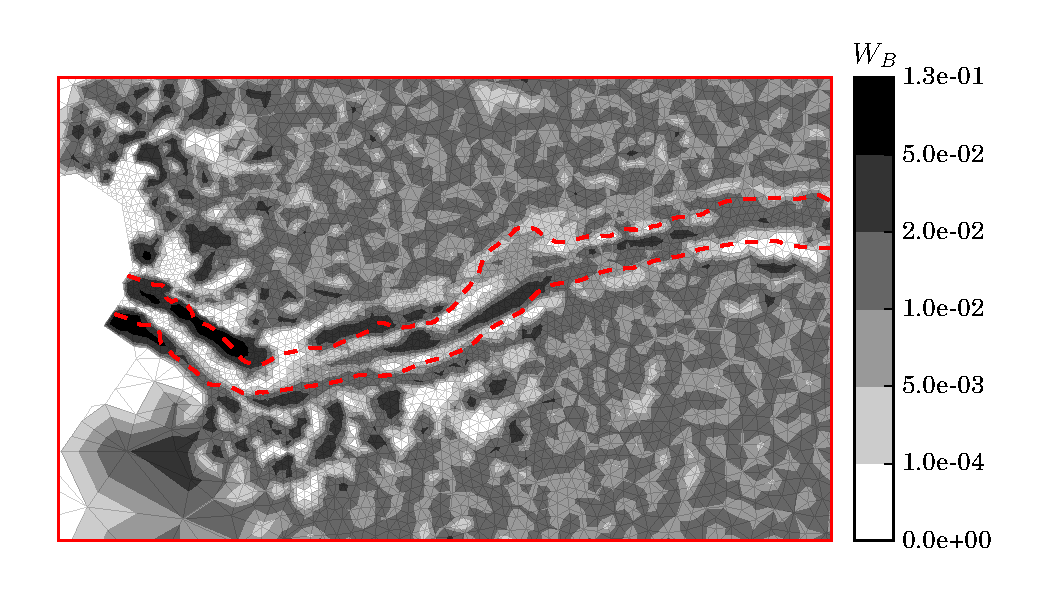
\includegraphics[width=0.48\linewidth]{images/internal_energy/jakob_results/inversion_Wc_0.01/W.pdf}
    \quad
    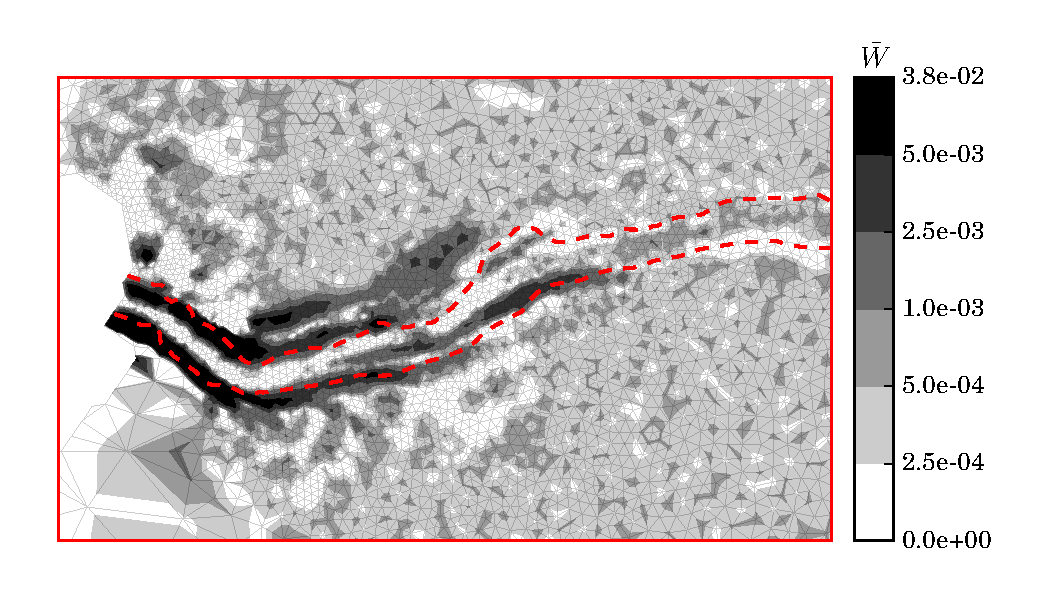
\includegraphics[width=0.48\linewidth]{images/internal_energy/jakob_results/inversion_Wc_0.01/Wbar.pdf}

    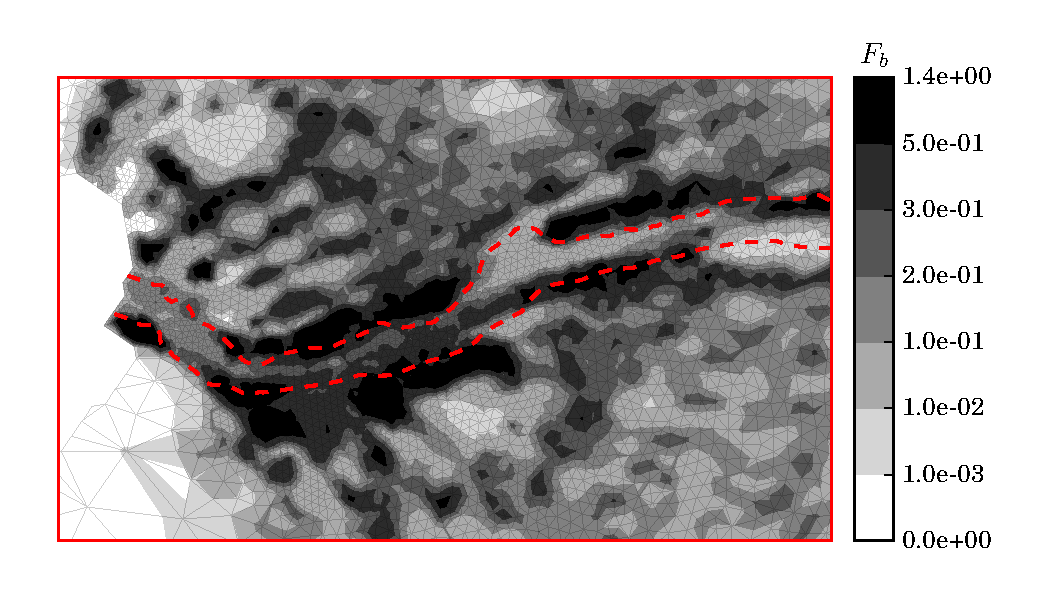
\includegraphics[width=0.48\linewidth]{images/internal_energy/jakob_results/inversion_Wc_0.01/Fb.pdf}
    \quad
    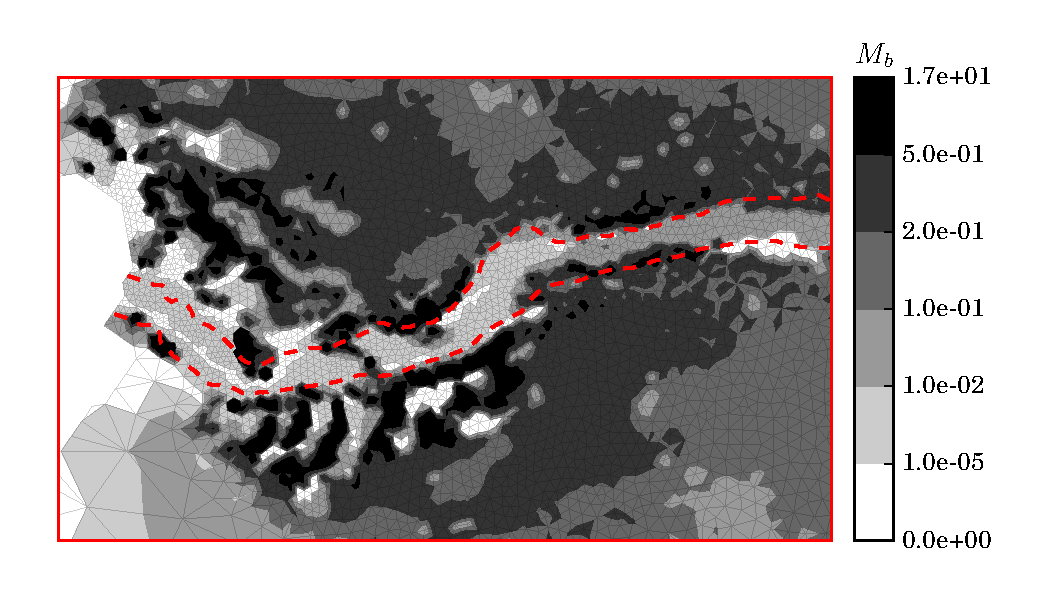
\includegraphics[width=0.48\linewidth]{images/internal_energy/jakob_results/inversion_Wc_0.01/Mb.pdf}
  \caption[Jakobshavn simulation results]{Results of TMC-inversion procedure \ref{tmc_da} with maximum basal water content $W_c = 0.01$ for region of Western Greenland's Jakobshavn Glacier.  The optimized surface velocity magnitude $\Vert \rankone{u}_S \Vert$ (top left), optimized basal traction $\beta$ (top right), ratio of ice column that is temperate (top middle left), velocity magnitude misfit (top middle right), basal water content $W$ (bottom middle left), vertically averaged water content (bottom middle right), optimized basal water discharge $F_b$ (bottom left) and basal melt rate $M_b$ (bottom right).  The dashed lines indicate the $-500$ m depth contour of basal topography $B$ depicted in Figure \ref{jakobshavn_topography}.}
  \label{jakobshavn_results}
\end{figure*}

\begin{figure*}
  \centering
    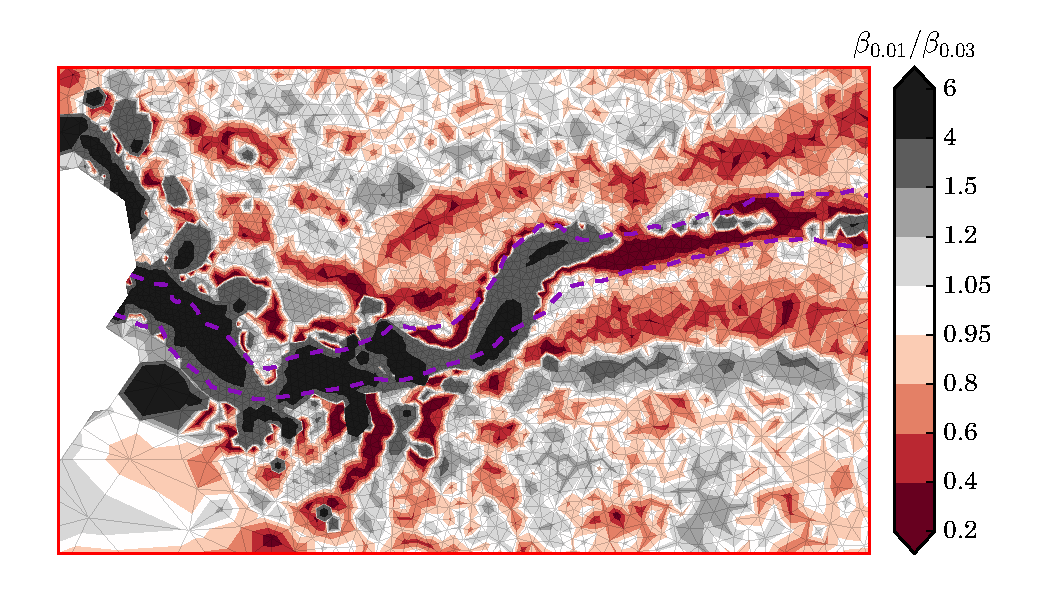
\includegraphics[width=\linewidth]{images/internal_energy/jakob_results/deltas/delta_beta.pdf}
  \caption[Effect of water content on basal traction]{Ratio of basal traction attained by Algorithm \ref{tmc_da} between using maximum basal water content $W_c = 0.01$ and $W_c = 0.03$.  These results were obtained using fewer momentum optimization iterations, resulting in traction fields which are more irregular than that depicted in Figure \ref{jakobshavn_results}.}
  \label{deltas}
\end{figure*}

\begin{figure*}
  
  \centering
  
  \begin{subfigure}[b]{0.32\linewidth}
    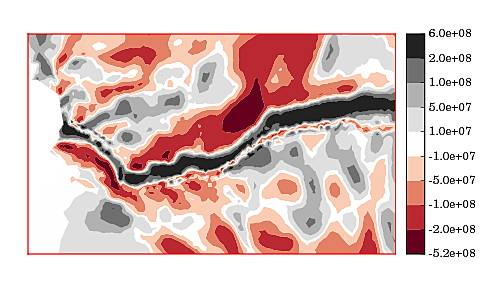
\includegraphics[width=\linewidth]{images/internal_energy/jakob_results/inversion_Wc_0.01/stress_balance/N_ii.jpg}
  \caption{$N_{ii}$}
  \label{N_ii}
  \end{subfigure}
  \begin{subfigure}[b]{0.32\linewidth}
    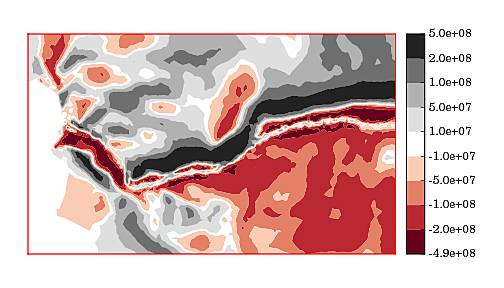
\includegraphics[width=\linewidth]{images/internal_energy/jakob_results/inversion_Wc_0.01/stress_balance/N_ij.jpg}
  \caption{$N_{ij}$}
  \label{N_ij}
  \end{subfigure}
  \begin{subfigure}[b]{0.32\linewidth}
    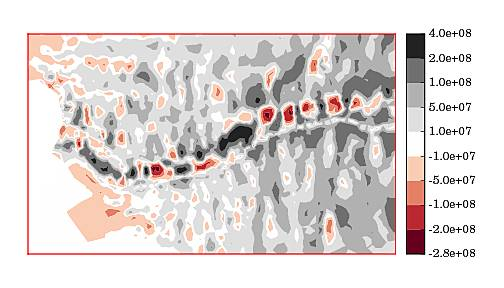
\includegraphics[width=\linewidth]{images/internal_energy/jakob_results/inversion_Wc_0.01/stress_balance/N_iz.jpg}
  \caption{$N_{iz}$}
  \label{N_iz}
  \end{subfigure}

  \begin{subfigure}[b]{0.32\linewidth}
    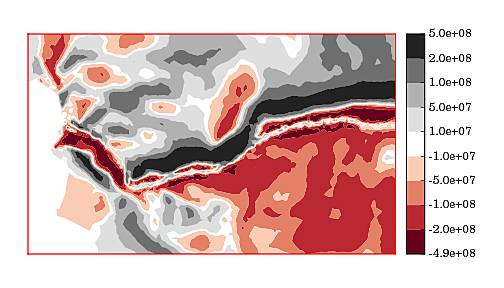
\includegraphics[width=\linewidth]{images/internal_energy/jakob_results/inversion_Wc_0.01/stress_balance/N_ji.jpg}
  \caption{$N_{ji}$}
  \label{N_ji}
  \end{subfigure}
  \begin{subfigure}[b]{0.32\linewidth}
    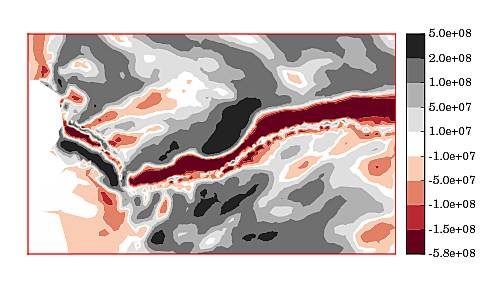
\includegraphics[width=\linewidth]{images/internal_energy/jakob_results/inversion_Wc_0.01/stress_balance/N_jj.jpg}
  \caption{$N_{jj}$}
  \label{N_jj}
  \end{subfigure}
  \begin{subfigure}[b]{0.32\linewidth}
    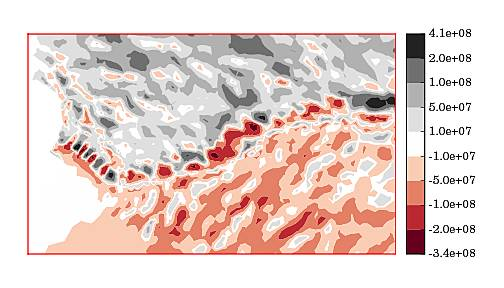
\includegraphics[width=\linewidth]{images/internal_energy/jakob_results/inversion_Wc_0.01/stress_balance/N_jz.jpg}
  \caption{$N_{jz}$}
  \label{N_jz}
  \end{subfigure}

  \begin{subfigure}[b]{0.32\linewidth}
    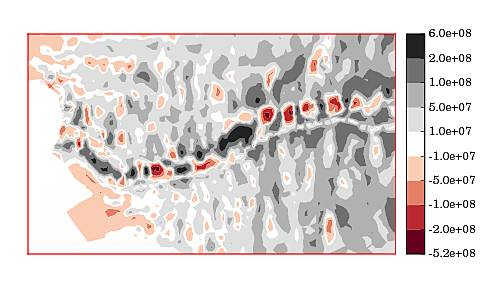
\includegraphics[width=\linewidth]{images/internal_energy/jakob_results/inversion_Wc_0.01/stress_balance/N_zi.jpg}
  \caption{$N_{zi}$}
  \label{N_zi}
  \end{subfigure}
  \begin{subfigure}[b]{0.32\linewidth}
    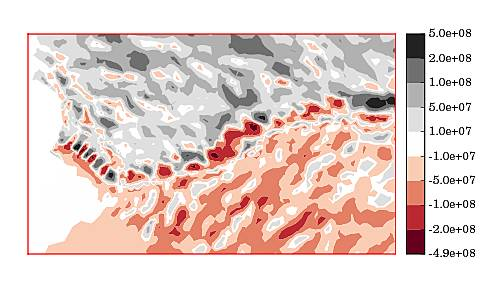
\includegraphics[width=\linewidth]{images/internal_energy/jakob_results/inversion_Wc_0.01/stress_balance/N_zj.jpg}
  \caption{$N_{zj}$}
  \label{N_zj}
  \end{subfigure}
  \begin{subfigure}[b]{0.32\linewidth}
    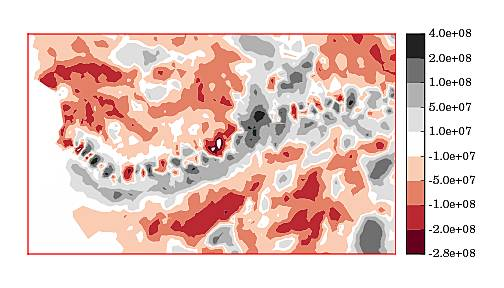
\includegraphics[width=\linewidth]{images/internal_energy/jakob_results/inversion_Wc_0.01/stress_balance/N_zz.jpg}
  \caption{$N_{zz}$}
  \label{N_zz}
  \end{subfigure}
  
  \begin{subfigure}[b]{0.32\linewidth}
    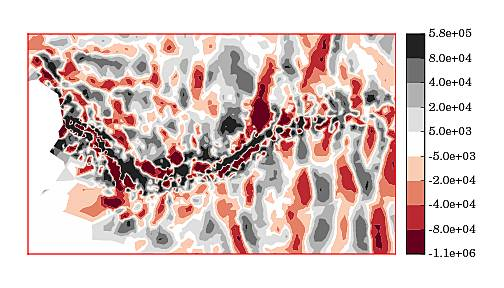
\includegraphics[width=\linewidth]{images/internal_energy/jakob_results/inversion_Wc_0.01/stress_balance/M_ii.jpg}
  \caption{$M_{ii}$}
  \label{M_ii}
  \end{subfigure}
  \begin{subfigure}[b]{0.32\linewidth}
    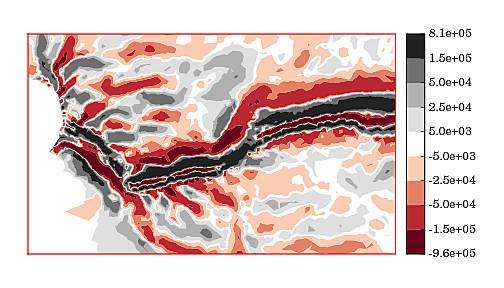
\includegraphics[width=\linewidth]{images/internal_energy/jakob_results/inversion_Wc_0.01/stress_balance/M_ij.jpg}
  \caption{$M_{ij}$}
  \label{M_ij}
  \end{subfigure}
  \begin{subfigure}[b]{0.32\linewidth}
    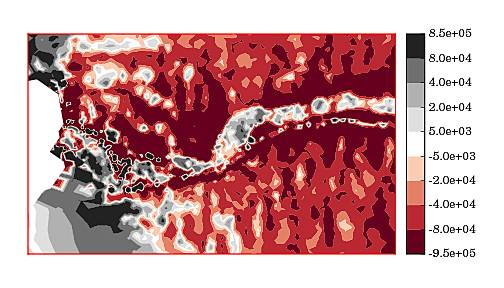
\includegraphics[width=\linewidth]{images/internal_energy/jakob_results/inversion_Wc_0.01/stress_balance/M_iz.jpg}
  \caption{$M_{iz}$}
  \label{M_iz}
  \end{subfigure}

  \begin{subfigure}[b]{0.32\linewidth}
    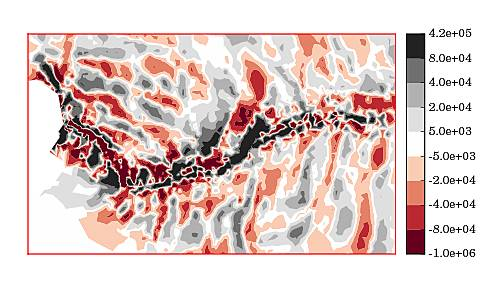
\includegraphics[width=\linewidth]{images/internal_energy/jakob_results/inversion_Wc_0.01/stress_balance/M_ji.jpg}
  \caption{$M_{ji}$}
  \label{M_ji}
  \end{subfigure}
  \begin{subfigure}[b]{0.32\linewidth}
    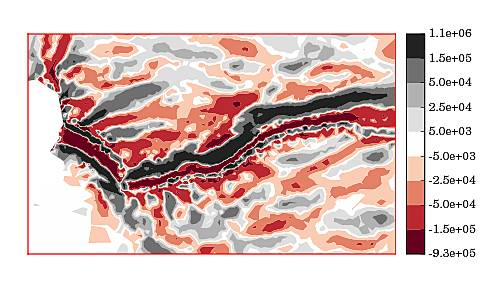
\includegraphics[width=\linewidth]{images/internal_energy/jakob_results/inversion_Wc_0.01/stress_balance/M_jj.jpg}
  \caption{$M_{jj}$}
  \label{M_jj}
  \end{subfigure}
  \begin{subfigure}[b]{0.32\linewidth}
    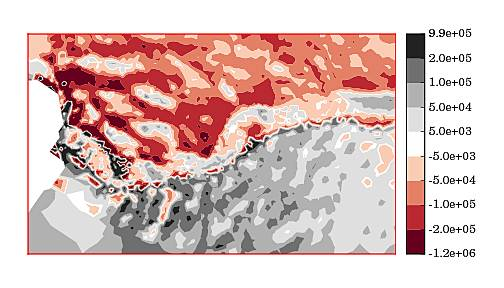
\includegraphics[width=\linewidth]{images/internal_energy/jakob_results/inversion_Wc_0.01/stress_balance/M_jz.jpg}
  \caption{$M_{jz}$}
  \label{M_jz}
  \end{subfigure}

  \begin{subfigure}[b]{0.32\linewidth}
    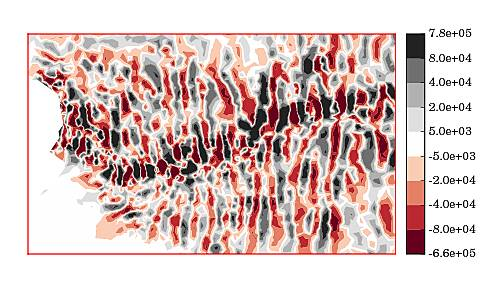
\includegraphics[width=\linewidth]{images/internal_energy/jakob_results/inversion_Wc_0.01/stress_balance/M_zi.jpg}
  \caption{$M_{zi}$}
  \label{M_zi}
  \end{subfigure}
  \begin{subfigure}[b]{0.32\linewidth}
    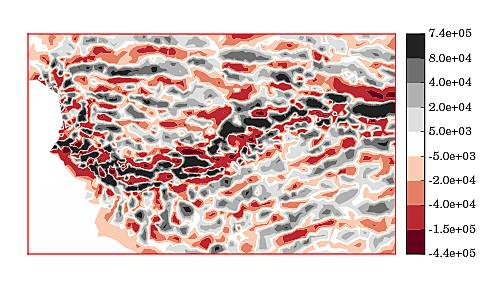
\includegraphics[width=\linewidth]{images/internal_energy/jakob_results/inversion_Wc_0.01/stress_balance/M_zj.jpg}
  \caption{$M_{zj}$}
  \label{M_zj}
  \end{subfigure}
  \begin{subfigure}[b]{0.32\linewidth}
    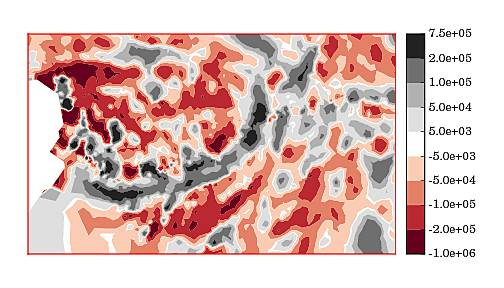
\includegraphics[width=\linewidth]{images/internal_energy/jakob_results/inversion_Wc_0.01/stress_balance/M_zz.jpg}
  \caption{$M_{zz}$}
  \label{M_zz}
  \end{subfigure}

  \caption[Jakobshavn membrane stress]{Membrane stress $N_{kk}$ and membrane-stress balance $M_{kk}$.}
  \label{jakobshavn_membrane_stress_balance}

\end{figure*}
